\begin{frame}{DNSSEC}
    \begin{itemize}
    \item public key infrastructure for DNS
    \item single set of root keys from ICANN/IANA
        \begin{itemize}
        \item no certificate authorities like web PKI
        \end{itemize}
    \item digital signature for each delegation to new servers
        \begin{itemize}
        \item delegation to new zone includes keys for that zone
        \item chain of signatures DNS client can check
        \item everything can still be cached
        \end{itemize}
    \item makes DNS messages a lot bigger
    \end{itemize}
\end{frame}


\begin{frame}{DNSSEC and missing records}
    \begin{itemize}
    \item tricky problem: validating `not present' responses
    \vspace{.5cm}
    \item DNSSEC has multiple options:
        \begin{itemize}
        \item signed `no result for X.Y.Z, type Q' message
        \item signed `no result between W.Y.Z and Z.Y.Z' message
        \item signed `no result with hash(?) = A < hash(X) < B = hash(?)' message
        \end{itemize}
    \item exercise: pro/cons?
    \end{itemize}
\end{frame}

\begin{frame}{DNSSEC deployment: validation}
    \begin{itemize}
    \item queries supporting validation: approx. 35\%
        \begin{itemize}
        \item from \url{https://stats.labs.apnic.net/dnssec/}
        \end{itemize}
    \item approx. 45\% recursive resolvers support 
        \begin{itemize}
        \item from \url{https://ithi.research.icann.org/}
        \end{itemize}
    \end{itemize}
\end{frame}

\begin{frame}{DNSSEC deployment: signing}
via \url{https://ithi.research.icann.org/graph-m11.html}: \\
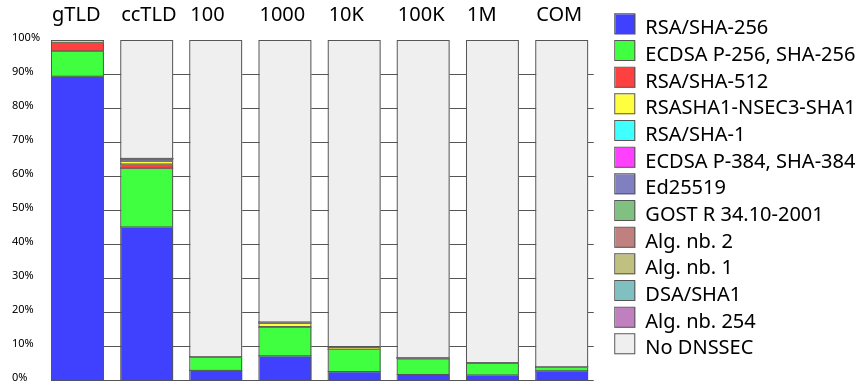
\includegraphics[height=0.8\textheight]{../dns/ithi-dnssec-deploy-oct-domains}
\end{frame}
